\documentclass{standalone}

%Til tikz billede
\usepackage{tikz}
\def\layersep{2.5cm}

\usetikzlibrary{shapes.multipart, matrix,chains,positioning,decorations.pathreplacing,shapes,arrows,arrows.meta}
\usetikzlibrary{arrows,decorations.pathmorphing,backgrounds,positioning,fit,petri}

% ggplot2 style tikz
\definecolor{obj}{gray}{0.95}
\definecolor{backG}{gray}{1}


\begin{document}
	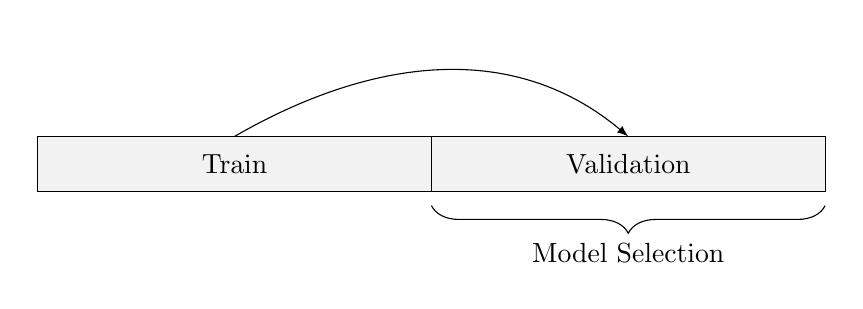
\begin{tikzpicture}[
	%  -{Stealth[length = 2.5pt]},
	start chain = going right,
	node distance = 0pt,
	MyStyle/.style={draw, minimum width=5cm, minimum height=2em, 
		outer sep=0pt, on chain,fill=obj},
	]
	\node [MyStyle] (1) {Train};
	\node [MyStyle] (2) {Validation};
	\begin{scope}[-{latex[length = 2.5pt]}]
	\draw (1.north) [out=30, in=140] to (2.north);
	\end{scope}
	\draw[fill=backG,decorate,decoration={brace, amplitude=10pt, raise=5pt, mirror}]
	(2.south west) to node[fill=backG,midway,below= 15pt] {Model Selection} (2.south east);
	
	\begin{pgfonlayer}{background}
	\node [fill=backG,fit=(current bounding box.north west) (current bounding box.south east)] {};
	\draw[step=1cm,white,very thin] (current bounding box.north west) grid (current bounding box.south east);
	\end{pgfonlayer}
	\end{tikzpicture}
\end{document}


%\chapter{Calculations}
%\label{chap:calc}
%\input{chapters/calc}